\documentclass[11pt]{article}
\usepackage{mynote2019}

% For Korean
\usepackage[hangul]{kotex} %%% 참고. hangul 옵션 제외 가능. finemath 추천.
\usepackage[utf8]{inputenc}

\pagestyle{fancy}
\lhead{Left Header here}
\rhead{
\includegraphics[clip=true,height=1em]{Figures/yourlogo.png}}
\lfoot{CopyLeft}
\cfoot{\thepage / \pageref{LastPage}}
\rfoot{Right footer}



%%----- 본문 시작 ----------------------------------------------------------------------------

\begin{document}

\singlespace

\mytitle{Network Coding}{\today}{Your Name}

\sectiontitle{Professional activities}  
\ud{mobile devices to discover and communicate with each other in close proximity. It also transforms these devices into social sensors, and allows programmers to \hla{rapidly develop locally and socially aware applications.} Several use cases demonstrate key concepts of Comm.unity.}

\udd{An avalanche of new technology promises to transform healthcare. You’ve heard a lot about it: Electronic medical records. New ways to mine genomic data to match patients with the right medicines. Everything from iPhone apps and robots to help you exercise or take your meds. Not to mention relatively “old” advances like digital imaging and telemedicine video hookups that connect those in remote places with doctors.}

\uddd{All this and a lot more fits under the broad umbrella of healthcare IT?and in Frank Moss’s view all of it (except maybe the robot part) falls far short of the mark of what technology should do for healthcare. You can find illustrations of many of his ideas?and he’s got a lot of them?in a corner of the MIT Media Lab, where Moss has set up a doctor’s table next to a living room arrangement as part of a research group called \mkc New Media Medicine.
}
 
\begin{figure}[htp]
   \centering
    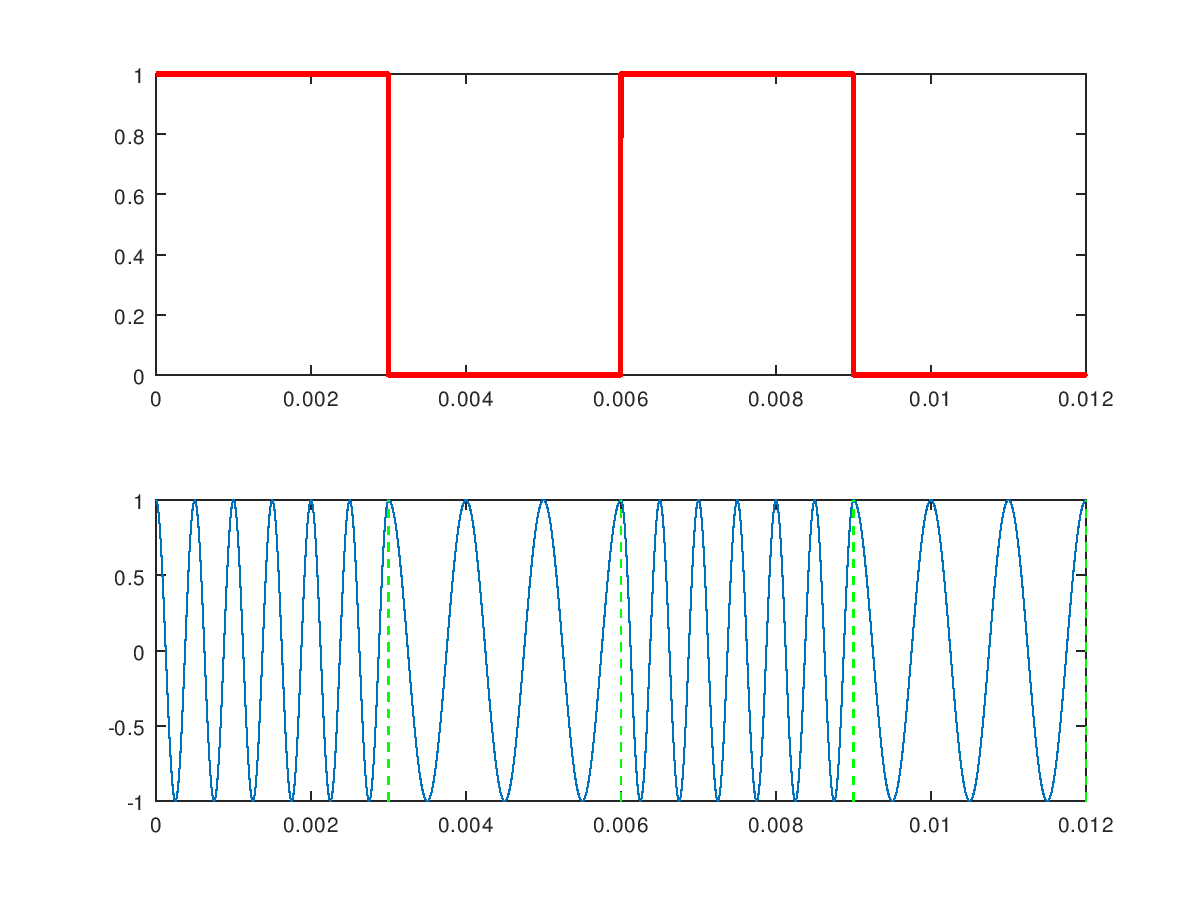
\includegraphics[scale=0.7]{Figures/fsk.png}
    \caption{NTP structure: Yellow(direct connection), Red(indirect connection)}
    \label{fig:ntp}
\end{figure}



%%----- 참고문헌은 여기에 ------------------------------------------------------------------------
%\newpage

\end{document}
